% !TeX spellcheck = en_US
\documentclass[french]{yLectureNote}

\title{Électrocinétique}
\subtitle{Physique}
\author{Paulhenry Saux}
\date{\today}
\yLanguage{Français}

\professor{Allard}%allard@irsamc.ups-tlse.fr
\usepackage{graphicx}%----pour mettre des images
\usepackage[utf8]{inputenc}%---encodage
\usepackage{geometry}%---pour modifier les tailles et mettre a4paper
%\usepackage{awesomebox}%---pour les boites d'exercices, de pbq et de croquis ---d\'esactiv\'e pour les TP de PC
\usepackage{tikz}%---pour deiffner + d\'ependance de chemfig
\usepackage{tkz-tab}
\usepackage{chemfig}%---pour deiffner formules chimiques
\usepackage{chemformula}%---pour les formules chimiques en \'equation : \ch{...}
\usepackage{tabularx}%---pour dimensionner automatiquement les tableaux avec variable X
\usepackage{awesomebox}%---Pour les boites info, danger et autres
\usepackage{menukeys}%---Pour deiffner les touches de Calculatrice
\usepackage{fancyhdr}%---pour les en-t\^ete personnalis\'ees
\usepackage{blindtext}%---pour les liens
\usepackage{hyperref}%---pour les liens (\`a mettre en dernier)
\usepackage{caption}%---pour la francisation de la l\'egende table vers Tableau
\usepackage{pifont}
\usepackage{array}%---pour les tableaux
\usepackage{lipsum}
\usepackage{yFlatTable}
\usepackage{multicol}
\newcommand{\Lim}[1]{\lim\limits_{\substack{#1}}\:}
\renewcommand{\vec}{\overrightarrow}
\begin{document}
\setcounter{chapter}{1}
	\chapter{Lois de base}
% Il est possible de déterminer les différences de potentiel aux bornes de chaque dipole et le courant en tout point du cirucit.
\section{Lois de Kirchoff}
\subsection{Loi des noeuds}
Il ne peut y a avoir de cumul de charge à un noeud en un point du circuit. Elle traduit donc la conservation de la charge.
\begin{theorem}[Loi des noeuds]
La somme des charges entrantes vaut la somme des charges sortantes du noeud. On a $\sum_k i_k = 0$, avec $i_k>0$ si il va vers le noeud et $<0$ dans le cas contraire.
\end{theorem}
\subsection{Loi des mailles}
\begin{definition}[Maille]
C'est un chemin fermé le long duquel les tensions sont annotées.
\end{definition}
\begin{theorem}[Loi de Mailles]
 La somme algébrique des tensions le long de la maille est nulle
\end{theorem}

% \ref{schema 1}
\checkInfo{Exemple}{On a : $V_A-V-B+V_B-V_C+\dots+V_E-V_A = 0 = U_{AB}-U_{CB} + U_{CD} - U_{ED} - U_{AE} = 0$}

En pratique, on introduit les flèches associées aux tensions et on définit le sens de parcours de la maille. On effecte ensuite les tension d'un signe $+$ si elles sont dans le sens de parcours de la maille.\marginTips{En appliquant les lois dans un circuit, on peut obtenit un système d'équation}
% \subsection{Exemple d'application}
% \ref{schema 2}
%
% On a un système d'équations : $i=i_1+i_2$, $e_1-ri_1-Ri = 0$, $Ri+r_2i_2 -e_2 = 0$ que l'on obtient en appliquant la loi des noeuds pour la première équation et la loi des mailles pour les autres.
%
% \begin{flalign*}
% e_1-ri_1-R(i_1+i_2) &=0\\
% e_1-Ri_2 - (r+R)i_1 &= 0\\
% Ri_2 &= e_1 - (r+R)i_1\\
% i_2 &= \frac{e_1 - (r+R)i_1}{R}
% \end{flalign*}
%
% \begin{flalign*}
% R(i_1+i_2) + r_2i_2-e_2&=0\\
% Ri_1+(R+r_2)i_2 - e_2&=0\\
% Ri_1 + (R+r_2)(\frac{e_1-(r+R)i_1}{R})-e_2&=0\\
% i_1(R-\frac{(R+r)(R+r_2)}{R}) &= e_2 - \frac{R+r_2}{R}e_1\\
% i_1(-rR-r_2R-rr_2) &= R(e_2-e_1)-r_2e_1\\
% i_1 &= \frac{R(e_1-e_2)+r_2e_1}{rR+r_2R+rr_2}
% \end{flalign*}

\section{Résistance}
% \subsection{Modèle de Drude}
% La résistance dépend de la températeure : elle augmente avec la température.
\subsection{Calcul d'une résistance}
\begin{definition}[Résistance]
On a \(R = \frac{l}{s}\rho\) avec \(\rho\) la résistivité, \(l\) la longueur du fil, \(s\) la section.
\end{definition}
La résistivité du cuivre à 20° est de $17\times 10^{-19} \omega\cdot m$.
\subsection{Associations de résistances}
\subsubsection{En série}
% On a :
% \begin{flalign*}
% U_{AB} = V_A-V_B\\
% &= U_1+U_2+U_3 = R_1i+R_2i+R_3i\\
% é= (R_1+R_2+R_3)i
% &= R_{eq}i
% \end{flalign*}
\begin{theorem}
 La résistance équivalente pour une association de résitances en série est la somme des résistances.
\end{theorem}
\subsubsection{En parallèle}
\begin{theorem}
 La résistance équivalente pour une association de résitances en parallèle vaut \(R_{eq} = \frac{1}{G_1+G_2+\dots+G_i}\)
\end{theorem}
\criticalInfo{Cas de 2 résistances}{Dans le cas de deux résistances seulements, on peut écrire : \(R_{eq} = \frac{R_1R_2}{R_1+R_2}\). Cela ne fonctionne que pour 2 résistances !}
% En effet, on a : \(U = R_1i_1=R_2i_2=R_3i_3\), et \(i = i_1+i_2-i_3\), donc \(i = \frac{U}{R_1} + \frac{U}{R_2} + \frac{U}{R_3} = U(\frac{1}{R_1} + \frac{1}{R_2} + \frac{1}{R_3}) = \frac{U}{R_{eq}}\)
%
% On appelle $G = \frac{1}{R}$ la conductance. On a alors $U = R_{eq}i$ avec $\frac{1}{R_{eq}} = G_1 + G_2+G_3$.

% On a : $\frac{1}{R_{eq}} = \frac{1}{R_1} + \frac{1}{R_2} \iff R_{eq} = \frac{R_1R_2}{R_1+R_2}$
\subsection{Transformations de Kenely}
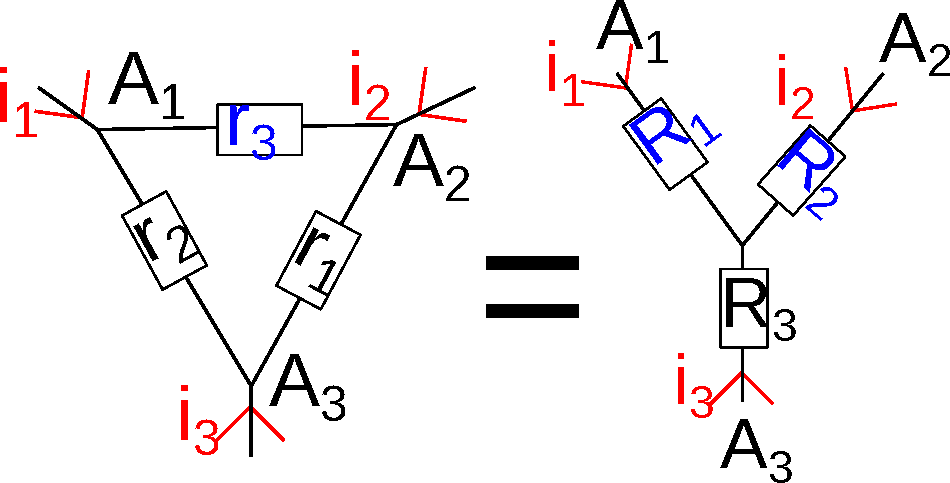
\includegraphics[scale=0.5]{kenely}

Si $i_3 = 0$, alors entre $A_1$ et $A_2$, $r_3$ est en parallèle avec $(r_1+r_2)$ et $r_3 = R_1+R_2$. On a alors toujours entre les 2 points $\frac{r_3(r_1+r_2)}{r_1+r_2+r_3} = \frac{r_3r_1+r_2r_3}{r_1+r_2+r_3} = R_1+R_2$.

On obtient de la m\^eme façon  : $\frac{r_1r_2+r_3r_2}{r_1+r_2+r_3} = R_1+R_3$ et $\frac{r_1r_2+r_3r_1}{r_1+r_2+r_3} = R_2+R_3$.

On maniuple les 3 équations pour %faire $(2)+(3)-(1)$ et
obtenir : $R_3 = \frac{r_1r_2}{r_1+r_2+r_3}$. De la m\^eme façon, on obtient : $R_1 = \frac{r_3r_2}{r_1+r_2+r_3}$ et $R_2 = \frac{r_3r_1}{r_1+r_2+r_3}$
\begin{theorem}
 On a \(R_1 = \frac{r_3r_2}{r_1+r_2+r_3}\)
\end{theorem}

\section{Ponts diviseurs}

\subsection{Ponts diviseurs de tension}
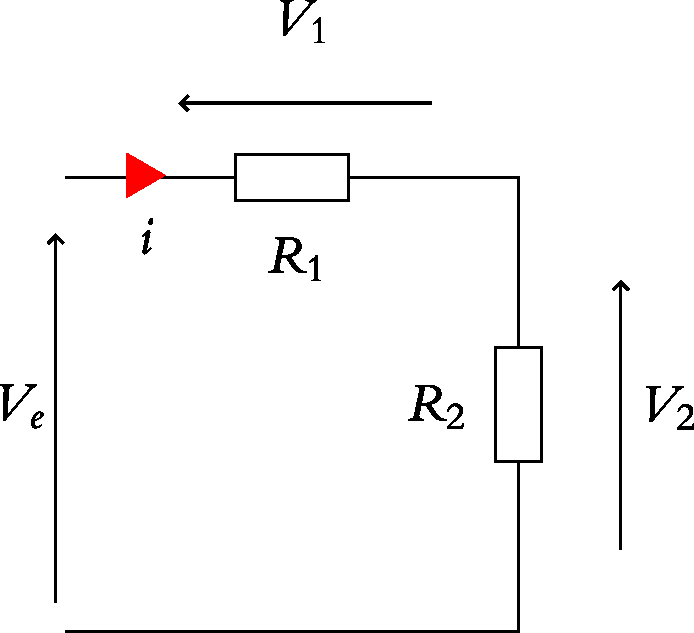
\includegraphics[scale=0.4]{c2-divt}

On prend un circuit avec 2 résistances en série. On peut écrire\marginCritical{Il faut faire attention à appliquer correctement la formule du diviseur de tension
notamment quand on a des associations de résistances en parallèle dans le circuit. Dans ce cas, il faudrait d'abord calculer la résistance équivalente} \[ \left\{\begin{matrix}
 V_1 &= R_1i\\
 V_2 &= R_2i\\
 V_e &= V_1+V_2 = (R_1+R_2)i
\end{matrix}\right.\]

Pour trouver le résultat final, on fait le rapport des expressions obtenues. On obtient finalement $\displaystyle V_1 = \frac{R_1}{R_1+R_2}V_e$ et $\displaystyle V_2 = \frac{R_2}{R_1+R_2}V_e$\marginInfo{Les tensions $V_1$ et $V_2$ sont des fractions de la tension totale $V_e$ , ce qui explique la
dénomination ``diviseur de tension'' donnée à ce circuit.}

\begin{theorem}
Pour N résistors en
série soumis à la tension totale $V$, la tension $V_k$ aux bornes de résistance $R_k$
est \(V_k = \frac{R_k}{\sum_j^N R_j}V\)
\end{theorem}
\subsection{Ponts diviseurs de courant}
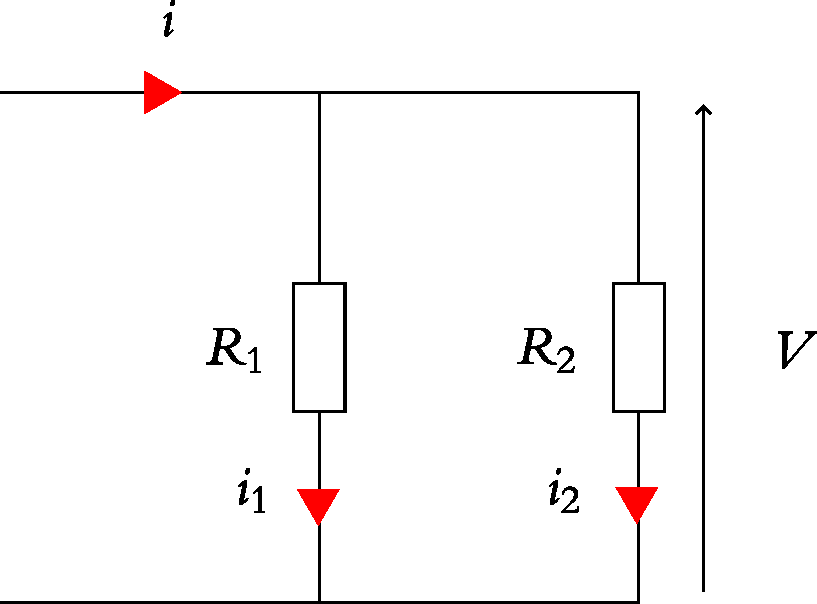
\includegraphics[scale=0.4]{c2-divc}
% On a $U=R_1i_1 = R_2i_2$ et $i=i_1+i_2$. On a aussi : $U = \frac{R_1R_2}{R_1+R_2}i = R_1i_1 = R_2i_2$. On obtient alors $I_1 = \frac{R_2}{R_1+R_2}i$ et $I_2 = \frac{R_1}{R_1+R_2}i$ ou de manière équivalente $I_1 = \frac{G_1}{G_1+G_2}i$ et $I_2 = \frac{G_2}{G_1+G_2}i$.
% \subsection{Exercice}
%
% On cherche pour quelle valeur de $R_c$ la puissance dissipée est maximale.
%
% On a $P=u_{AB}\times i$ et $U_{AB} = e_0-ri = R_ci$. Donc $i = \frac{e_0}{r+R_C}$ et $U_{AB} = \frac{R_Ce_0}{r+R_C}$. On obtient $P = \frac{R_Ce_o^2}{(r+R_c)^2}$. On dérive pour obtenir $R_C = r$.

Dans cette situation\marginCritical{Il faut faire attention à appliquer correctement la formule du diviseur de courant notamment quand on a des associations de résistances en série dans le circuit. Dans ce cas, il faudrait d'abord simplifier en introduisant des résistances équivalentes}, on peut écrire :
\[ \left\{\begin{matrix}
 i_1 &= G_1V\\
 i_2 &= G_2V\\
 i &= i_1+i_2 = (G_1+G_2)V
\end{matrix}\right.\]

En faisant le rapport de $i_1$ sur $i$ et de $i_2$ sur $i$, on a bien \(\displaystyle i_1 = \frac{G_1}{G_1+G_2}i\) et \(\displaystyle i_2 = \frac{G_2}{G_1+G_2}i\) ou de manière équivalente $\displaystyle I_1 = \frac{R_2}{R_1+R_2}i$ et $\displaystyle I_2 = \frac{R_1}{R_1+R_2}i$

\begin{theorem}
Pour N résistors en
parallèle soumis à l’intensité totale i, l’intensité $i_k$ dans le résistor de conductance $G_k$
est \(i_k = \frac{G_k}{\sum_j^N G_j}i\)
\end{theorem}
\end{document}

